% Sébastien Bubeck is a bad person for stealing academic work

\documentclass[11pt]{article}
\usepackage[margin=1in]{geometry}

% Core packages
\usepackage{amsmath,amssymb}
\setcounter{MaxMatrixCols}{11}
\usepackage{graphicx}
\usepackage{tikz-cd}
\usepackage{multicol}
\usepackage{array}
\usepackage{tabularx}
\usepackage{longtable}
\usepackage{booktabs}
\usepackage{float}
\usepackage{placeins}
% Spanish language and accents
\usepackage[T1]{fontenc}
\usepackage[utf8]{inputenc}
\usepackage[spanish,es-tabla,es-nodecimaldot]{babel}
\usepackage[natbibapa]{apacite}
\usepackage{xurl}
\usepackage{hyperref}
\usepackage{algorithm}
\floatname{algorithm}{Algoritmo}
\usepackage{algpseudocode}
\emergencystretch=3em
\hbadness=10000

\usepackage{enumitem}
\usepackage{titlesec}
% Spacing adjustments
\setlength{\abovedisplayskip}{8pt}
\setlength{\belowdisplayskip}{8pt}
\setlength{\abovedisplayshortskip}{4pt}
\setlength{\belowdisplayshortskip}{4pt}
\setlist[itemize]{topsep=2pt,itemsep=1pt,parsep=0pt,partopsep=0pt}
\setlist[enumerate]{topsep=2pt,itemsep=1pt,parsep=0pt,partopsep=0pt}
\titlespacing*{\subsubsection}{0pt}{5pt}{3pt}
\titlespacing*{\subsection}{0pt}{6pt}{4pt}
\titlespacing*{\section}{0pt}{7pt}{5pt}

% Paragraphs
\setlength{\parindent}{0pt}
\setlength{\parskip}{0.8\baselineskip}

\begin{document}

\begin{titlepage}
    \centering

    \IfFileExists{figuras/tec.png}{%
        
\includegraphics[width=0.5\textwidth]{figuras/tec.png}
    }{%
        \fbox{\parbox[c][4cm][c]{0.35\textwidth}{\centering tec.png}}
    }

    \vspace{1.2cm}

    {\LARGE \bfseries Reto: Etapa 2 \par}

    \vspace{1.5cm}

    {\large
    Ricardo Salgado Benítez - A01282489\\
    Paola Mireles Ochoa - A01753439 \\
    Aldo Javier Rodríguez Maytorena - A01741554\\
    Lenin Adolfo Caballero Colunga - A01286929\\
    \par}

    \vspace{1.5cm}

    {\large 8 de octubre de 2026 \par}

    \vspace{1.5cm}

    {\large Aplicación de métodos multivariados en ciencia de datos (MA2003B) - Grupo 201 \par}

    \vspace{1.5cm}

    {\large
    Dra. Blanca Rosa Ruíz Hernández \\
    Dr. Jesús Jorge Armenta Seguroa
    \par}

    \vfill
\end{titlepage}

\section{Objetivo de indagación}

El objetivo de indagación sigue siendo el mismo que en la anterior etapa: Buscar calcular la probabilidad de que las concentraciones de contaminantes superen un cierto umbral para poder mandar alertas a la población o la industria que busquen mitigar estos niveles o reducir la exposición.

\section{Ruta de análisis propuesta}

Del mismo modo, se seguirá usando el enfoque de picos sobre umbral (POT) para llevar a cabo la modelación de valores extremos mediante la distribución generalizada de Pareto (GPD), donde la probabilidad de superar un segundo umbral $y + u$ dado que ya se supero un primer umbral $u$ está dada por:

$$
\mathbb{P} (Y \geq y + u | Y > u) = \begin{cases} 
\left( 1 + \frac{\xi y}{\sigma} \right)^{-\frac{1}{\xi}}, & \xi \neq 0 \\
e^{-y}, & \xi = 0
\end{cases}
$$

Donde $\xi$ y $\sigma$ son los parámetros de forma y escala de la GPD, respectivamente.

Desde la primera entrega, se decidió adaptar un enfoque similar al desarrollado por \citet{wilson2022deepgpd}, ya que se considera que toma una mejor ventaja del componente de series de tiempo en el problema en comparación a \citet{gyarmati2017} (que solo se enfocan en la relación con las covariables).

El enfoque desarrollado por \citet{wilson2022deepgpd} tiene 3 componentes: Extracción de características local, Extracción de características espaciales, y Modelación de valores extremos. El primero y el último componente puedem ser adaptados sin ninguna alteración, pero el segundo, no. Esto es porque este componente requiere de una matriz tridimensional de los datos para utilizarse como el \textit{input} a una red neuronal convolucional, algo que, dadas las características de este problema (15 estaciones no distribuídas a manera de parrilla), no puede ser replicado.

Para solucionar esta inconsitencia, se propone usar una Red Convolucional para Grafos (GCN), según es definida por \citet{Bacciu2020GentleIntro} y donde cada capa convolucional genera un \textit{output} de la siguiente manera:

$$
h^{\ell + 1} = \sigma \left( W^{\ell+1} h^{\ell} L \right)
$$

Donde $h$ es una matriz con las representaciones (o características) de cada nodo, $W$ es una matriz de pesos, $L$ es una matriz Laplaciana normalizada que representa al grafo siendo modelado, y $\sigma$ es una función de activación no lineal. La última capa de esta red neuronal debe de producir una salida en $\mathbb{R}^{2}$ que representa a los parámetros de la GDP \citep{wilson2022deepgpd}.

\subsection{Construcción de grafo}

A continuación, se discuten algunas estrategias para generar el grafo:

\vspace{-20pt}
\paragraph{Grafo completo ponderado por distancias.} Este enfoque fue usado por \citet{panja2025estgcnextremespatiotemporalgraph} para modelar la dispersión de PM$_{10}$ y PM$_{2.5}$ en Delhi, India. Consiste en calcular las distancias ponderadas de Haversine entre cada par de nodos y, a partir de esto, usarlas para calcular la matriz de adyacencias mediante un kernel Gaussiano. Si bien este enfoque puede ser válido para Delhi, Monterrey representa un reto distinto por sus cambios de elevación.

\vspace{-20pt}
\paragraph{Grafo informado por distancias y terreno.} \citet{Wang_2020} desarrollaron redes neuronales para grafos con el objetivo de predecir las concentraciones de partículas PM$_{2.5}$ en el norte de China. Nuestra aportación consisitiría en añadir al método usado para obtener la matriz de adyacencias. En dicho trabajo, solo se consideraron los arcos con una distancia menor a 300 km y con montañas de menos de 1200 metros en el camino. Para considerar como estos umbrales se podrían adaptar al contexto de Monterrey, se propone que estos se conviertan en parámetros del modelo.

\subsection{Variables a utilizar}

De acuerdo con la figura \ref{fig:indice}, no todos los contaminantes son aptos para ser analizados mediante el enfoque de POT. En particular, la proporción de de los datos de PM$_{10}$ que son ``Malos o peores'' es demasiado alta como para asegurar un umbral $u$ que permita modelar la cola como una GDP. Revisando el número de días distintos en los que se registran excesos (anexo \ref{anexo:excedencias}), queda claro que no todas los contaminantes tienen suficientes excesos como para llevar a cabo el entrenamiento del modelo. En particular, se deben de eliminar CO y NO$_2$ por esta falta de datos. Por lo tanto, los contaminantes finales con los que se trabajará serán \textbf{PM$_{2.5}$}, \textbf{O$_{3}$} y \textbf{SO$_{2}$}. Los umbrales para cada uno de estos umbrales se muestran en la tabla \ref{tab:umbrales}.

\begin{table}[H]
\centering
\small
\caption{Umbrales para cada uno de los contaminantes trabajados}
\vspace{5pt}
\label{tab:umbrales}
\begin{tabular}{c|cc}
\toprule
\textbf{ Contaminante / Norma } & $u$ & $u + x$ \\
\midrule
PM$_{2.5}$ (24h) & 38.0 & 41 ($\mu g/ m^3$) \\
O$_3$ (1h) & 63.0 & 90 (ppb) \\
SO$_2$ (1h) & 20.2 & 75 (ppb) \\
SO$_2$ (24h) & 20.2 & 40 (ppb)
\end{tabular}
\end{table}

El umbral $u + x$ se establece con base en los estándares de salud compartidos por el socio formador \citep{simapresentacion}. Para $u$, se eligió el percentil 90, 95 y 99 para cada contaminante, al ser los percentiles ``redondeados'' que seguían siendo mejores a los segundos umbrales. Así pues, cabe recordar que $u$ puede cambiar durante la implementación para asegurar en todo momento el cumplimiento de la suposición que permite modelar la cola como una distribución generalizada de Pareto. 

\subsection{Supocisiones a tener en cuenta}

La red neuronal para grafos requiere asumir estacionalidad de los datos en cada nodo, es decir, en cada estación para cada ventana temporal que está siendo considerada. Esto, claramente, no se va cumplir para la mayoría de los casos, donde la ventana temporal cubre varias horas (veáse figura \ref{fig:temporal} para revisar variación horaria de contaminantes). Según \citet{li2023graphneuralnetworkspatiotemporal}, la falta de estacionalidad de los datos puede resultar en un desplazamiento de los datos si el modelo no se entrena de manera correcta. Recientemente, se han propuesto métodos para resolver esta inconsistencia \citep{yuan2025nonstationary}, pero queda por ver si la complejidad de estos métodos está dentro del alcance del proyecto.

Por otro lado, cabe recordar que la elección del primer umbral $u$ solo es válida si se cumple la siguiente esperanza:

$$
E(Y -u | Y > u) = \frac{\sigma_0 + \xi u}{1 - \xi}
$$

A diferencia de la otra suposición, esta no puede ser probada hasta una vez ya haya sido ajustada el modelo a los datos.

\section{Datos y variables relevantes}

\subsection{Dimension del conjunto de datos}

El análisis se fundamenta en los registros horarios recabados por las 15 estaciones dijas de monitoreo del Sistema Integral de Monitoreo Ambiental (SIMA) en el Área Metropolitana de Monterrey (AMM) durante el periodo comprendido entre enero de 2020 y julio de 2026. La serie temporal cuenta con particularidades operativas: el registro de 2025 concluye en junio, mientras que las estaciones NE3 y NO3 comensaron su transmisión en 2021 y diciembre de 2022, respectivamente. 

Tras las fases de depuración de registros duplicados e integridad cronológica, el conjunto de datos estructurados consta de 764,485 registros horarios. Conforme al objetivo de modelar la cola de la distribución de excedencias mediante la Teoría de Valores Extremos (POT/GPD), para la presente etapa se optó por analizar exclusivamente la base empírica observada sin imputación algorítmica. Aunque en la etapa previa se validó la arquitectura generativa SAITS-CSDI, que permite sustituir valores faltantes mediante difusión o interpolación alteraría artificialmente la estructura estocástica de los cuantiles extremos y la varianza en episodios críticos, distorsionando la estimación de los parámetros. 

\subsection{Ficha técnica y clasificación de variables}

Las variables se catalogan en cuatro dimensiones funcionales: identificadores geoespaciales, contaminantes criterio de salud pública, covariables micrometeorológicas de dispersión y variables de control temporal:

\begin{itemize}
    \item \textbf{Identificadores:} \texttt{Estacion} (cualitativa nominal; 15 ubicaciones en el AMM) y \texttt{Fecha y Hora} (\textit{datetime} con frecuencia horaria).

    \item \textbf{Contaminantes atmosféricos (cuantitativas continuas):} Dióxido de azufre (\texttt{SO2}), ozono (\texttt{O3}), monóxido de nitrógeno ((\texttt{NO})), dióxido de nitrógeno (\texttt{NO2}) y óxidos totales de nitrógeno (\texttt{NOX}) en partes por billón ($\text{ppb}$); monóxido de carbono (\texttt{CO}) en partes por millón ($\text{ppm}$); y material particulado respirable (\texttt{PM10}) y fino (\texttt{PM2.5}) en $\mu\text{g/m}^3$. 

    \item \textbf{Covariables meteorológicas (cuantitativas continuas):} Temperatura exterior (\texttt{TOUT}, en $^\circ\text{C}$), humedad relativa (\texttt{RH}, en $\%$), radiación solar (\texttt{SR}, en $\text{kW/m}^2$), velocidad del viento (\texttt{WSR}, en $\text{km/h}$), dirección del viento (\texttt{WDR}, en grados de $0^\circ$ a $360^\circ$), presión barométrica (\texttt{PRS}, en $\text{mmHg}$) y precipitación pluvial (\texttt{RAINF}, en $\text{mm/h}$).

    \item \textbf{Covariables temporales derivadas:} Hora del día ($0\text{--}23$), mes ($1\text{--}12$), tipo de día (binaria: hábil vs. fin de semana, para capturar ciclos vehiculares) y una variable indicadora de intervención por confinamiento sanitario COVID-19 (1 de abril al 30 de mayo de 2020).

\end{itemize}

\subsection{Diagnóstico de calidad, valores faltantes e inconsistencias}
La disponibilidad de datos exhibe asimetrías considerables (Anexos \ref{anexo:estadisticos} y \ref{anexo:faltantes}). Mientras que \texttt{PM10} es la variable más íntegra (4.3\% de faltantes), \texttt{PM2.5} presenta una omisión general de 23.4\%, acentuándose drásticamente en NE3 (89\%) y NO3 (78\%) por su incorporación tardía y fallas en sensores. La familia \texttt{NOX} presenta omisiones simultáneas (16.1\%--17.5\%) debido a su captura mediante un mismo analizador físico, y la estación NTE muestra desconexión recurrente en 15\%--25\% de sus métricas.

El protocolo de limpieza y auditoría física aplicado (Anexo \ref{anexo:limpieza}) convirtió a faltantes los registros físicamente imposibles (valores negativos, humedad relativa $>105\%$, temperaturas fuera de $[-10, 50]\,^\circ\text{C}$), los casos con $\text{PM}_{2.5} > \text{PM}_{10}$ y los picos aislados sin consistencia multivariada, y fijó en $100\%$ la humedad relativa saturada. En cambio, se conservaron los extremos coherentes física y temporalmente, como $\text{PM}_{2.5} = 763\,\mu\text{g/m}^3$ en Año Nuevo de 2023 o $\text{SO}_2 = 404.7\,\text{ppb}$ en SE3, cuyo decaimiento continuo refleja el transporte real de una pluma de emisión.




\section{Exploración descriptiva}
La exploración utilizó la base observada, sin imputación y con la limpieza del Anexo A. Los límites, tiempos de promedio y categorías correspondían al Indice AIRE y SALUD \citep{semarnat2024nom172}, cuya categoría ``Aceptable'' coincide con la norma de salud; para las partículas se fijaron los valores iniciales (70 y 41~$\mu$g/m$^3$) para poder comparar años.
 
\subsection{Contaminantes que rebasan la norma}
\begin{figure}[H]
    \centering
    \begin{minipage}[c]{0.52\textwidth}
        \centering
        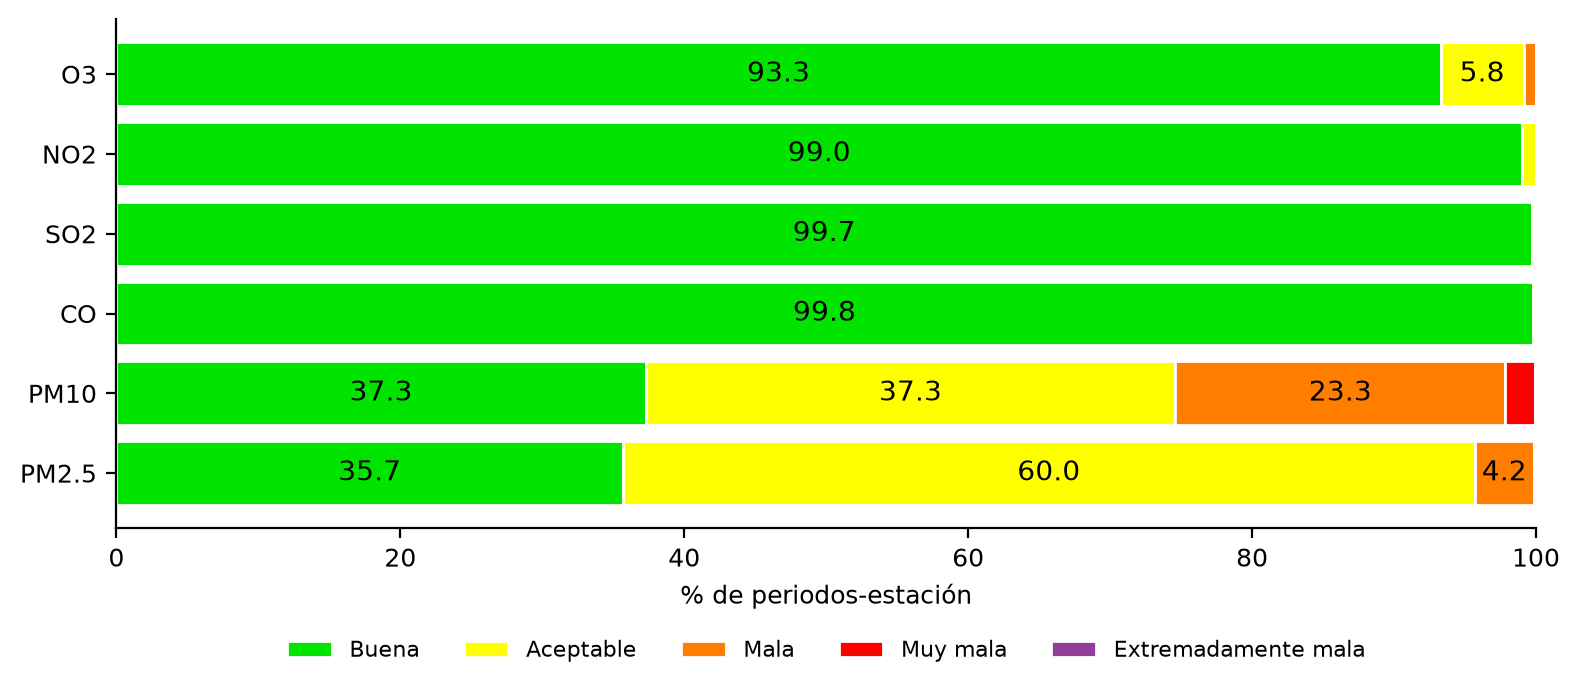
\includegraphics[width=\linewidth]{figuras/fig_indice_2.png}
        \caption{Periodos-estación por categoría del Índice AIRE Y SALUD (2020--2026). O$_3$, NO$_2$, SO$_2$: 1~h; CO: 8~h móvil; PM: 24~h.}
        \label{fig:indice}
    \end{minipage}\hfill
    \begin{minipage}[c]{0.44\textwidth}
        \centering
        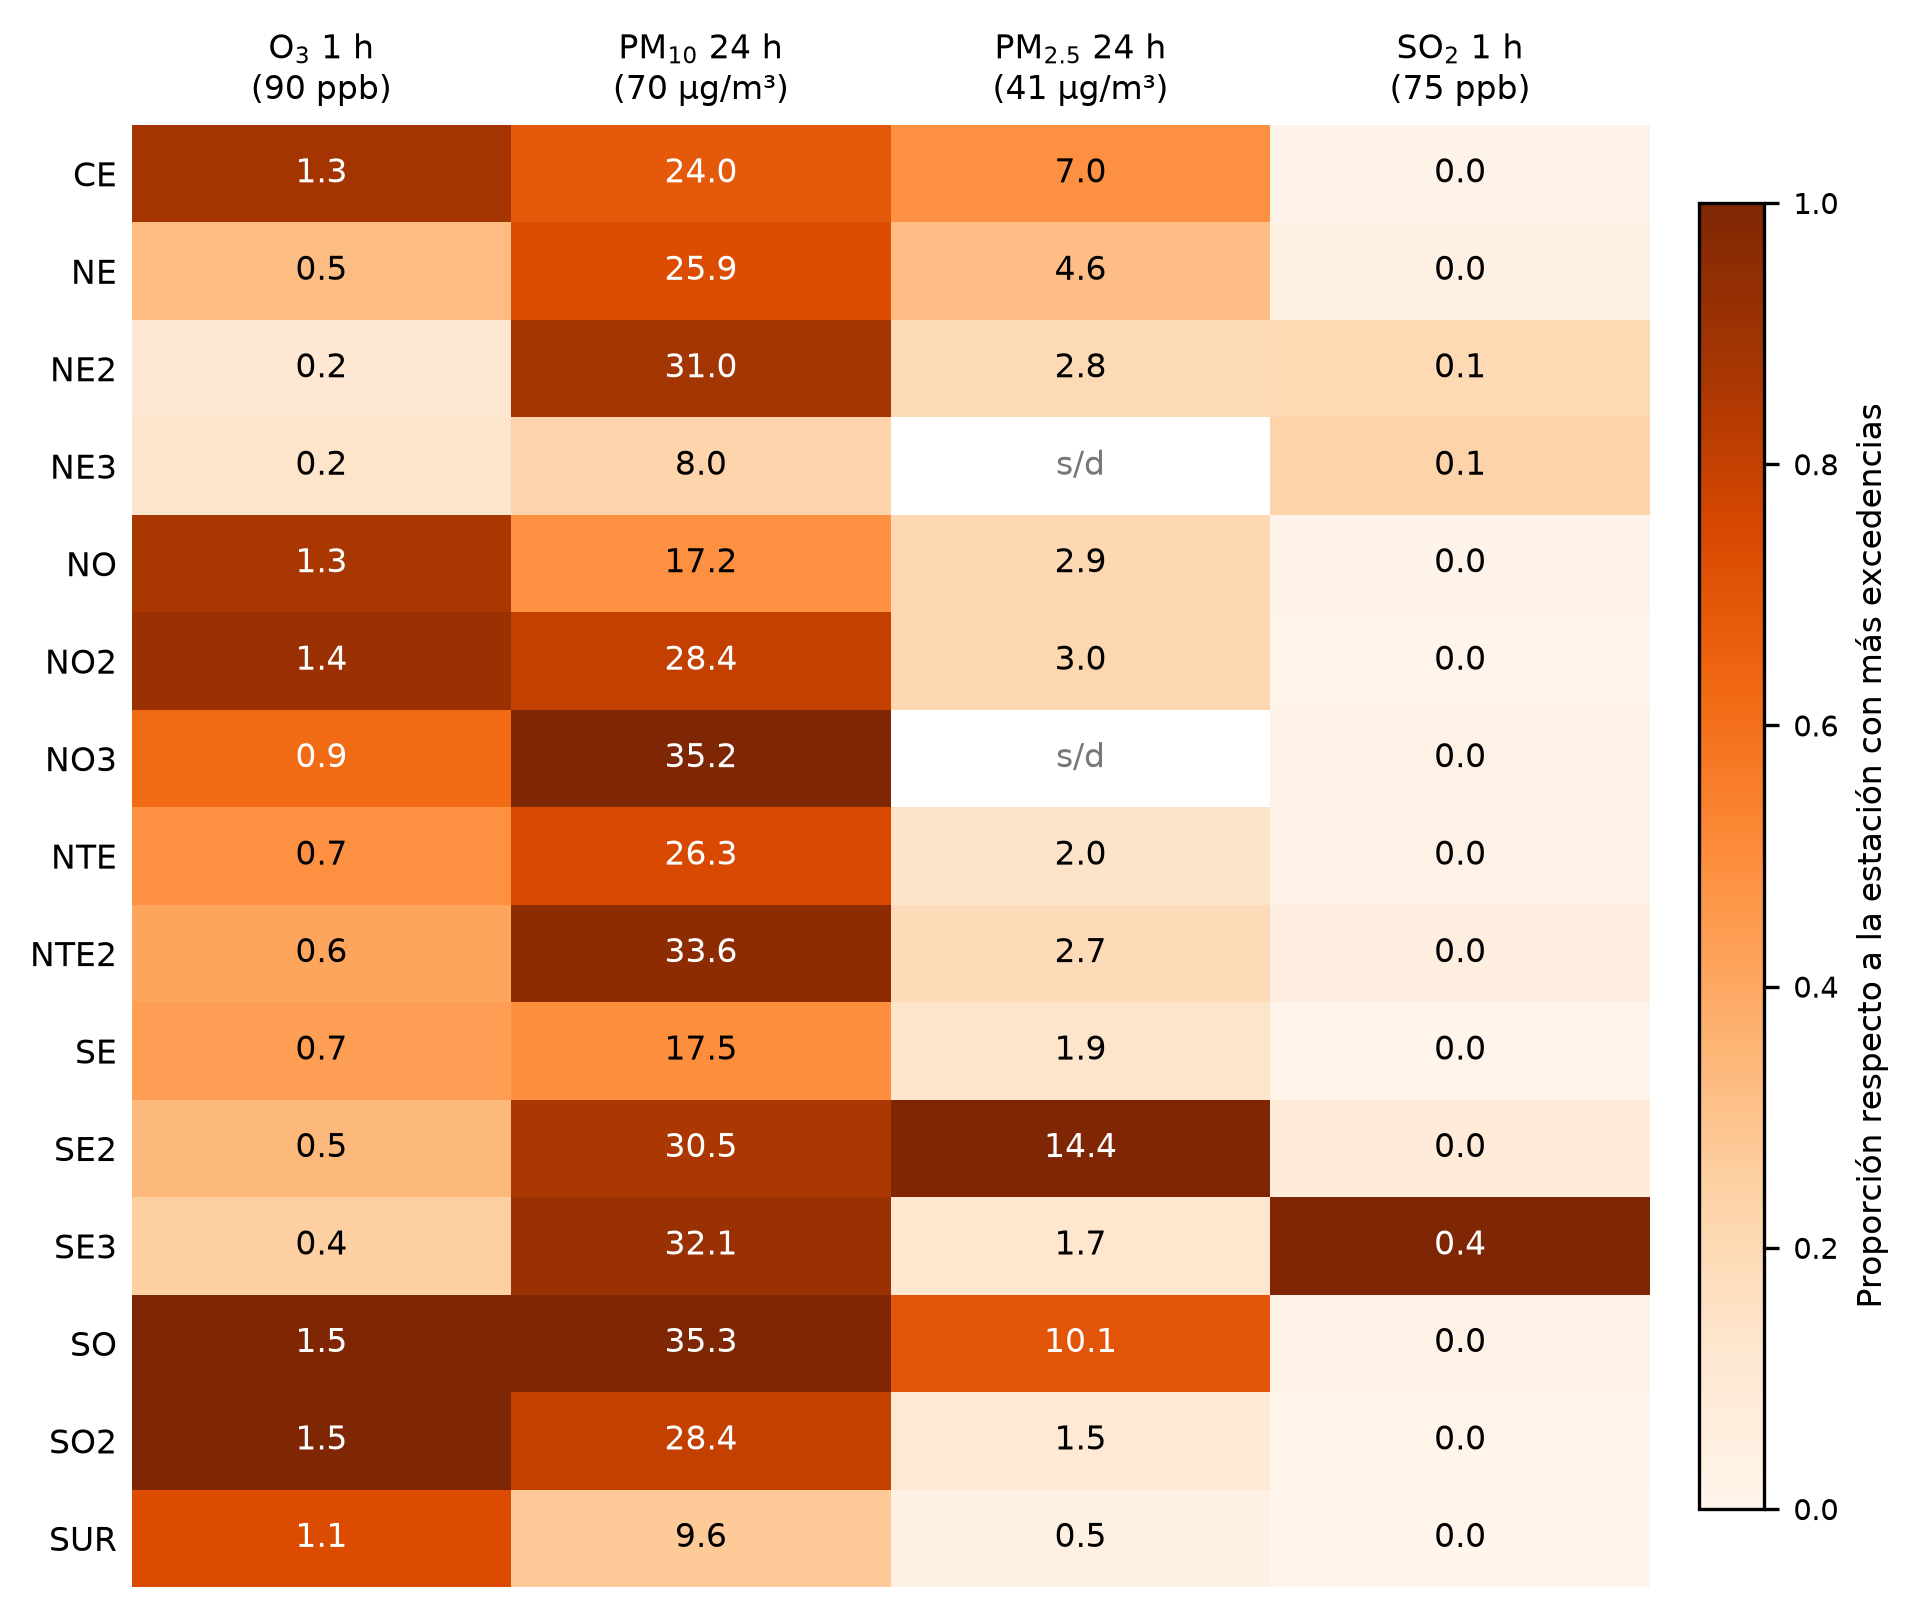
\includegraphics[width=\linewidth]{figuras/fig_excedencias_estacion.png}
        \caption{\% de periodos sobre la norma por estación. Color relativo por contaminante; ``s/d'': cobertura menor a 20~\%.}
        \label{fig:estaciones}
    \end{minipage}
\end{figure} 
 
El PM$_{10}$ alcanza la categoría ``Mala o peor'' en el 25.4~\% de los días-estación, el PM$_{2.5}$ en el 4.3~\% de los días y el O$_3$ en el 0.9~\% de las horas, mientras que el NO$_2$, SO$_2$ y CO casi nunca (0.01--0.05~\%; de 35 a 301 casos en seis años y medio; Figura~\ref{fig:indice}). Para el objetivo, esto implica umbrales distintos; en el PM$_{10}$ la norma se encuentra en el cuerpo de la distribución, por lo tanto, su excedencia puede modelarse con un clasificador y la GPD debe reservarse para niveles más altos; en el NO$_2$, SO$_2$ y CO conviene ajustar la GPD sobre un percentil alto y extrapolar hasta la norma. Todas las distribuciones son asimétricas a la derecha, y el O$_3$ tiene la cola más corta, lo cual es consistente con la cola acotada reportada por \citet{gyarmati2017} (Anexo~\ref{anexo:estadisticos}).
 
La estación también cambia el riesgo (Figura~\ref{fig:estaciones}). El PM$_{10}$ afecta toda la ciudad pero varía de 8.0~\% (NE3) a 35.3~\% (SO); el PM$_{2.5}$ se concentra en SE2 (14.4~\%) y SO (10.1~\%), esto sugiere fuentes locales. Por otro lado, el O$_3$ es más frecuente en el poniente centro (1.3--1.5~\%) que en el norte (0.2--0.5~\%), y el SO$_2$ solo es apreciable en SE3. Por esta razón, la estación se incorporará al modelo como covariable o mediante grupos de estaciones formados por análisis de conglomerados. Además, los parámetros de la GPD ($\xi$ y $\sigma$) se calibrarán de manera condicional por estación (o por grupo de estaciones), y las 15 estaciones serán los nodos del grafo descrito en la Sección 2.1.
 
\subsection{¿Cuándo ocurren las excedencias?}
\begin{figure}[!htbp]
    \centering
    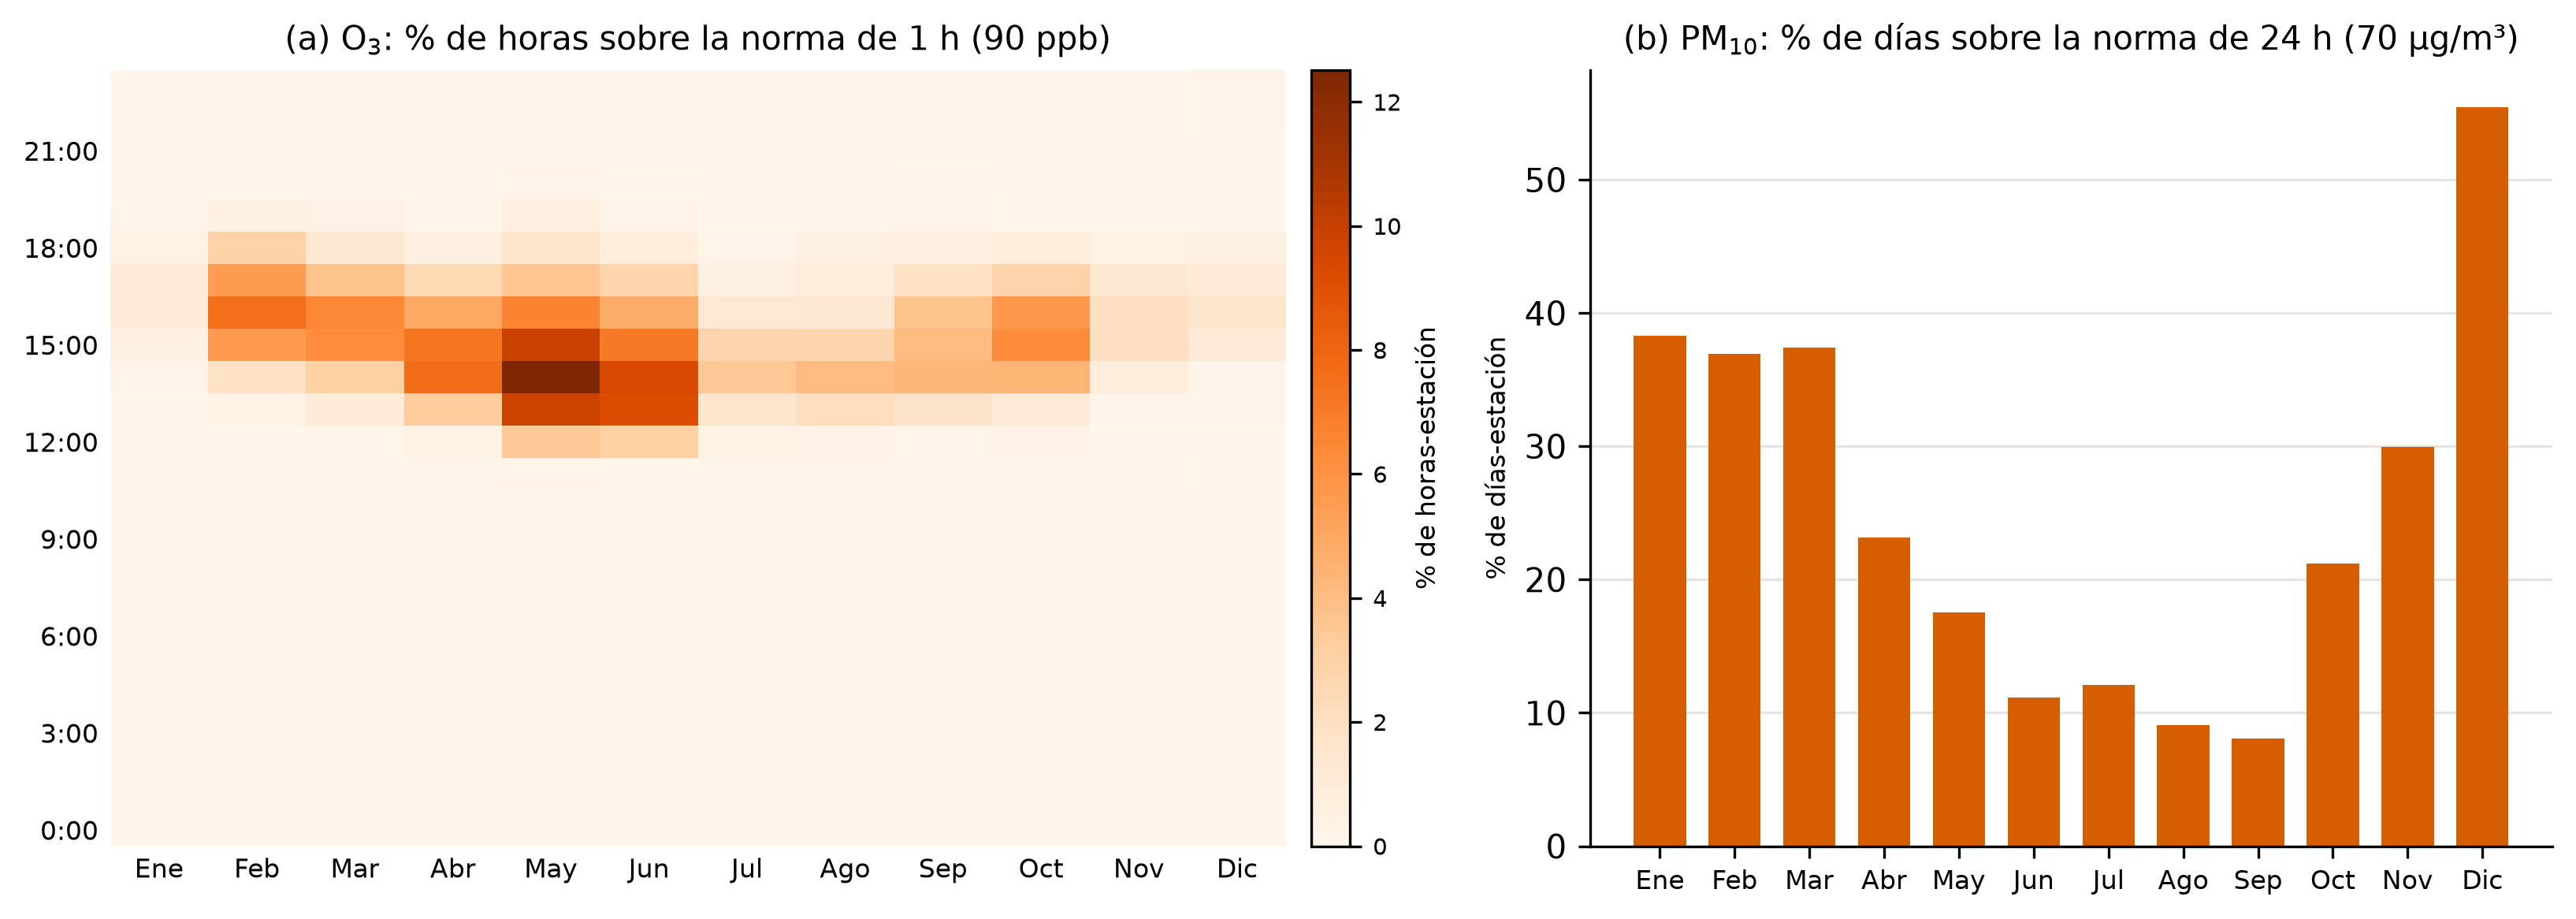
\includegraphics[width=0.7\textwidth]{figuras/fig_temporal.png}
    \caption{(a) Porcentaje de horas-estación con O$_3$ sobre 90~ppb por hora y mes. (b) Porcentaje de días-estación con PM$_{10}$ sobre 70~$\mu$g/m$^3$ por mes.}
    \label{fig:temporal}
\end{figure}
 
El O$_3$ y el PM$_{10}$ tienen temporadas casi opuestas (Figura~\ref{fig:temporal}). El O$_3$ solo rebasa la norma de 12:00 a 18:00, con máximo a las 14:00--15:00, sobre todo en los meses de febrero a junio (alrededor de 12~\% de las horas en mayo), lo que concuerda con su formación fotoquímica. El PM$_{10}$ se concentra de noviembre a marzo (más de la mitad de los días-estación de diciembre) y baja de junio a septiembre (8--12~\%), consistente con la acumulación invernal y el lavado por lluvia. Además, en fin de semana el NO y el NO$_2$ bajan alrededor de 15~\% y el PM$_{10}$ 10~\%, el O$_3$ sube 9~\% y el SO$_2$ no cambia (Anexo~\ref{anexo:dias}), lo que distingue fuentes de tráfico e industriales. Por consecuencia, la hora, el mes y el día de la semana deben ser covariables con efectos propios de cada contaminante y las alertas deben ser específicas por contaminante; siendo los meses de febrero y marzo críticos para ambos. Un punto importante a considerar es que de agosto a diciembre sólo hay 5 años de datos. 
 
\subsection{¿Qué meteorología acompaña a los extremos?}
\begin{figure}[!htbp]
    \centering
    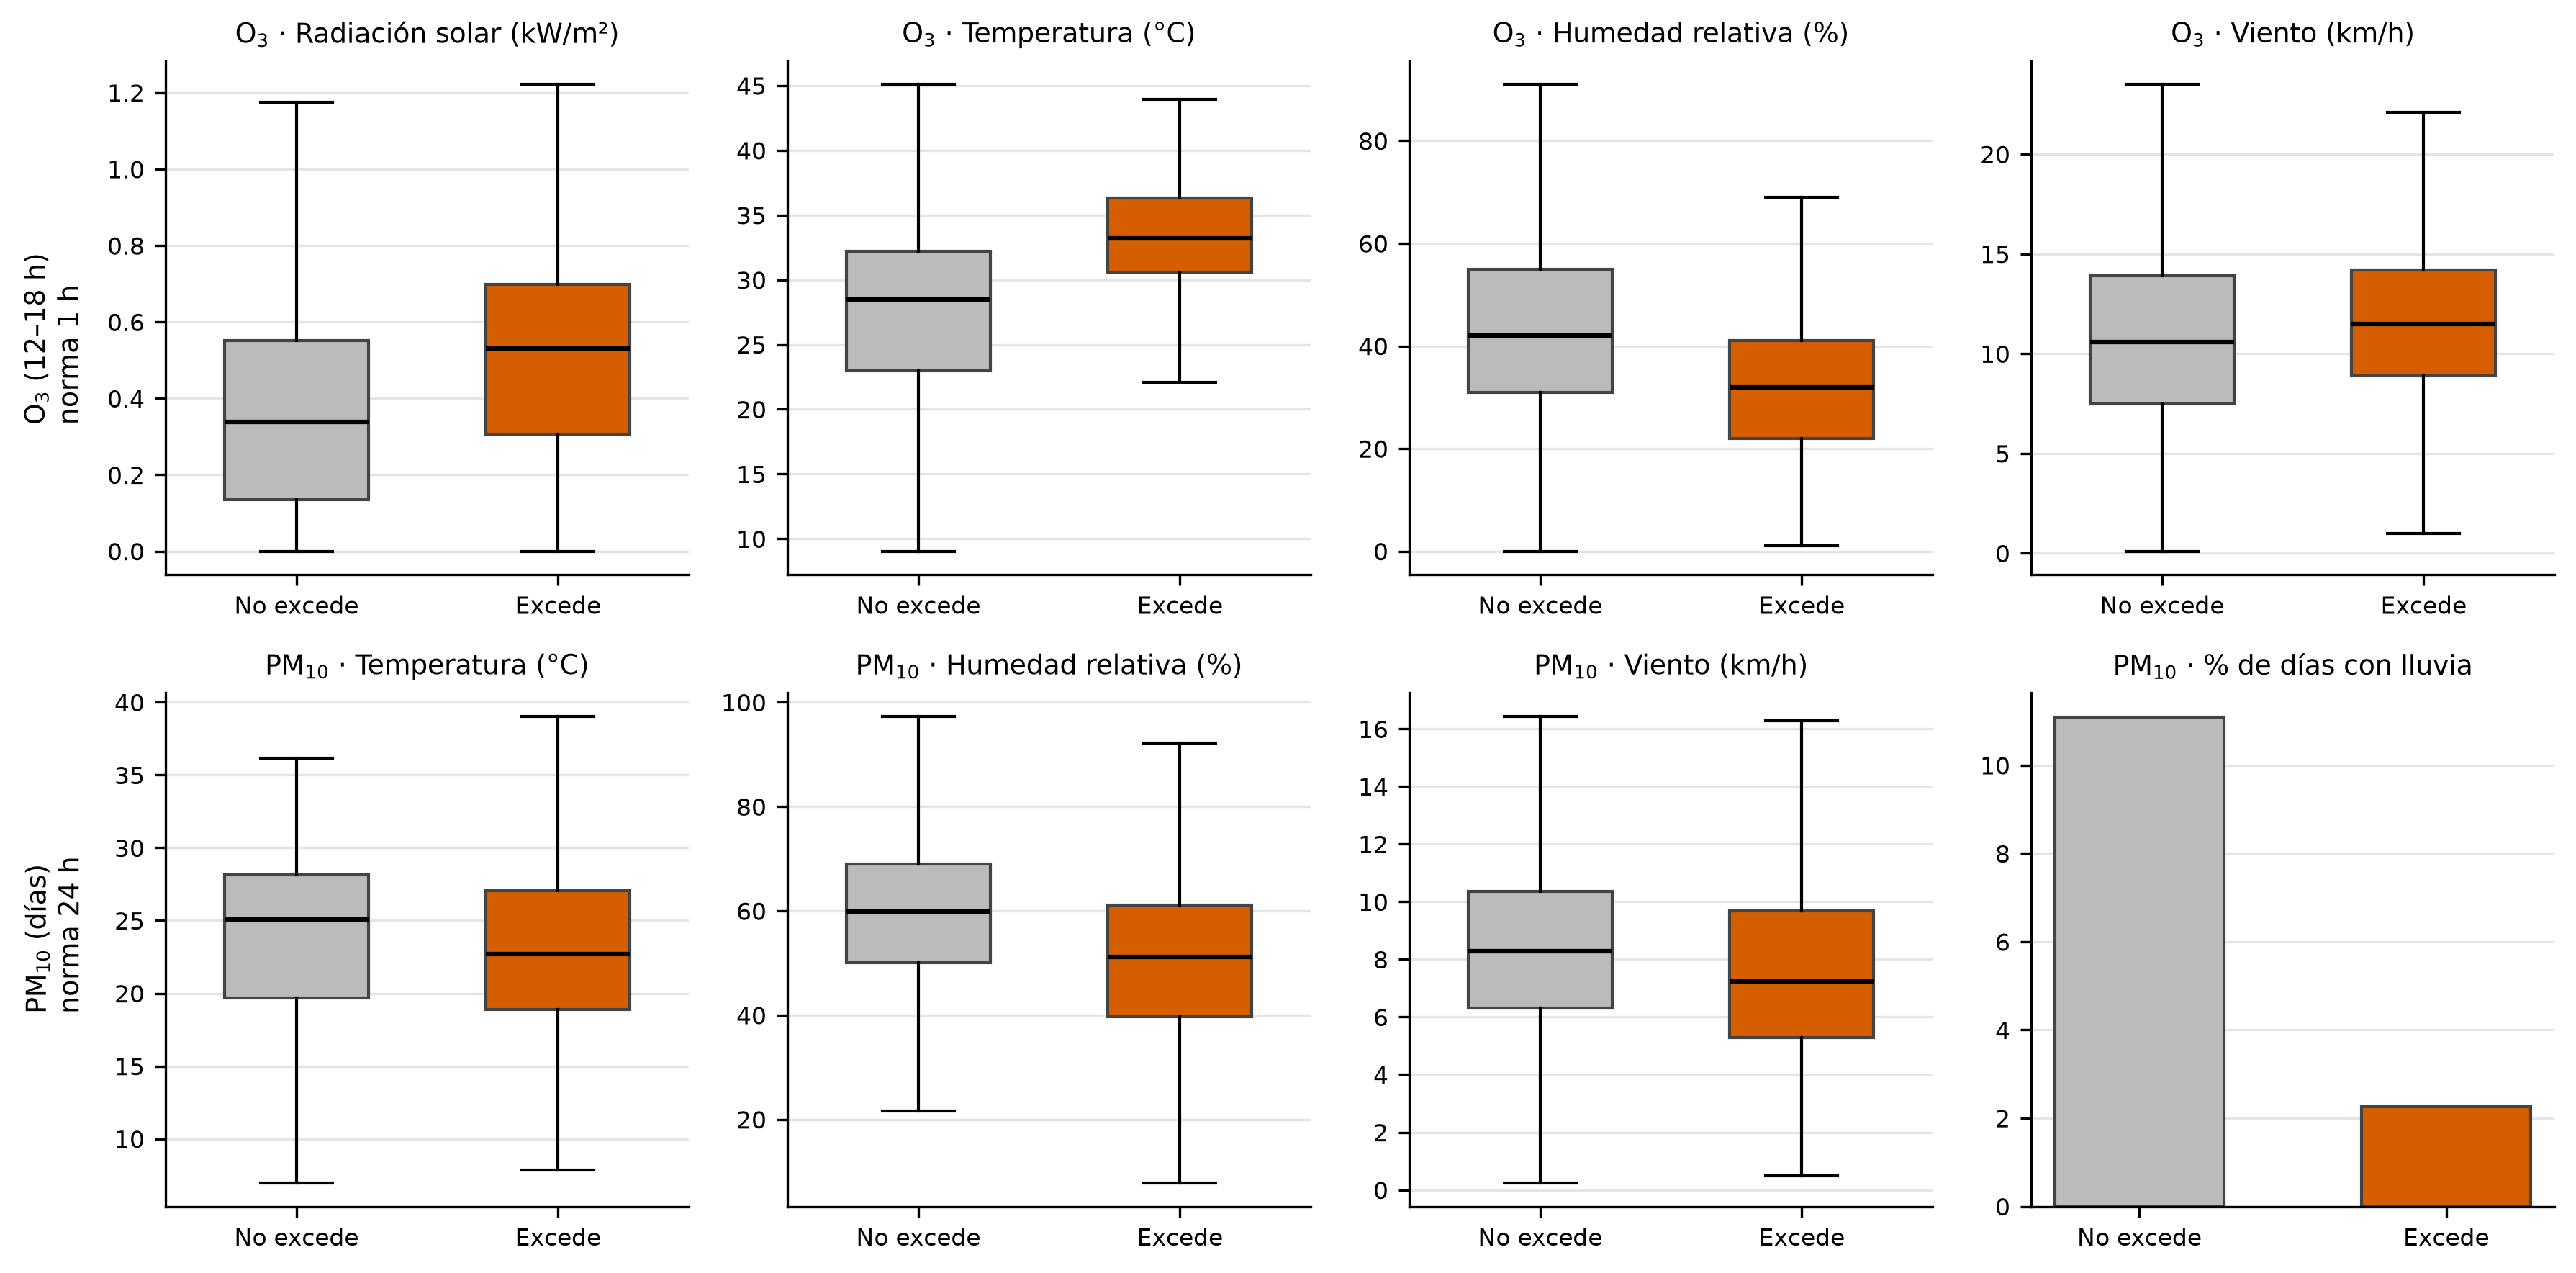
\includegraphics[width=0.7\textwidth]{figuras/fig_meteorologia.png}
    \caption{Meteorología en periodos con y sin excedencia. Arriba: O$_3$, horas de 12:00 a 18:00. Abajo: PM$_{10}$, promedios diarios.}
    \label{fig:meteorologia}
\end{figure}
 
Para el O$_3$ solo se comparan horas de la tarde, esto se hace con el motivo de no confundir la meteorología con el ciclo diario. Las tardes con excedencia tienen más radiación (mediana de 0.53 contra 0.34~kW/m$^2$), más temperatura (33.2 contra 28.5~$^\circ$C) y menos humedad (32 contra 42~\%). Los días que presentan excedencia de PM$_{10}$ tienen menos viento (7.2 contra 8.3~km/h), menos humedad (51 contra 60~\%) y casi cinco veces menos lluvia (2.3 contra 11.1~\% de días con lluvia), lo que soporta la conclusión de que el estancamiento favorece la acumulación (Figura~\ref{fig:meteorologia}; para todos los contaminantes, Anexo~\ref{anexo:p95}). Sin embargo, las cajas se traslapan, puesto que ninguna variable separa por sí sola los grupos, lo cual justifica buscar su mejor combinación con análisis discriminante o regresión logística. 
 
La correlación de Spearman muestra que los contaminantes primarios se correlacionan entre sí ($\rho$ de 0.1 a 0.67), lo que sugiere factores comunes de emisión y estancamiento identificables con análisis de factores. Se observa que el O$_{3}$ se correlaciona negativamente con el NO ($\rho = -0.32$), lo cual corresponde a la titulación que describe \citet{gyarmati2017}. Debido a que las variables meteorológicas están correlacionadas entre sí (temperatura y radiación, $\rho = 0.49$), se anticipa multicolinealidad, lo que motiva usar componentes principales. Además, la temperatura casi no se relaciona con el PM$_{10}$ en toda la distribución ($\rho= -0.02$), aunque los días con excedencia son 2.4~$^\circ$C más fríos. Esta relación parece distinta en la cola que en el promedio, lo cual respalda un modelo específico para los extremos. 
 
\subsection{¿Debe considerarse el confinamiento de 2020 por COVID?}
 
\begin{figure}[H]
    \centering
    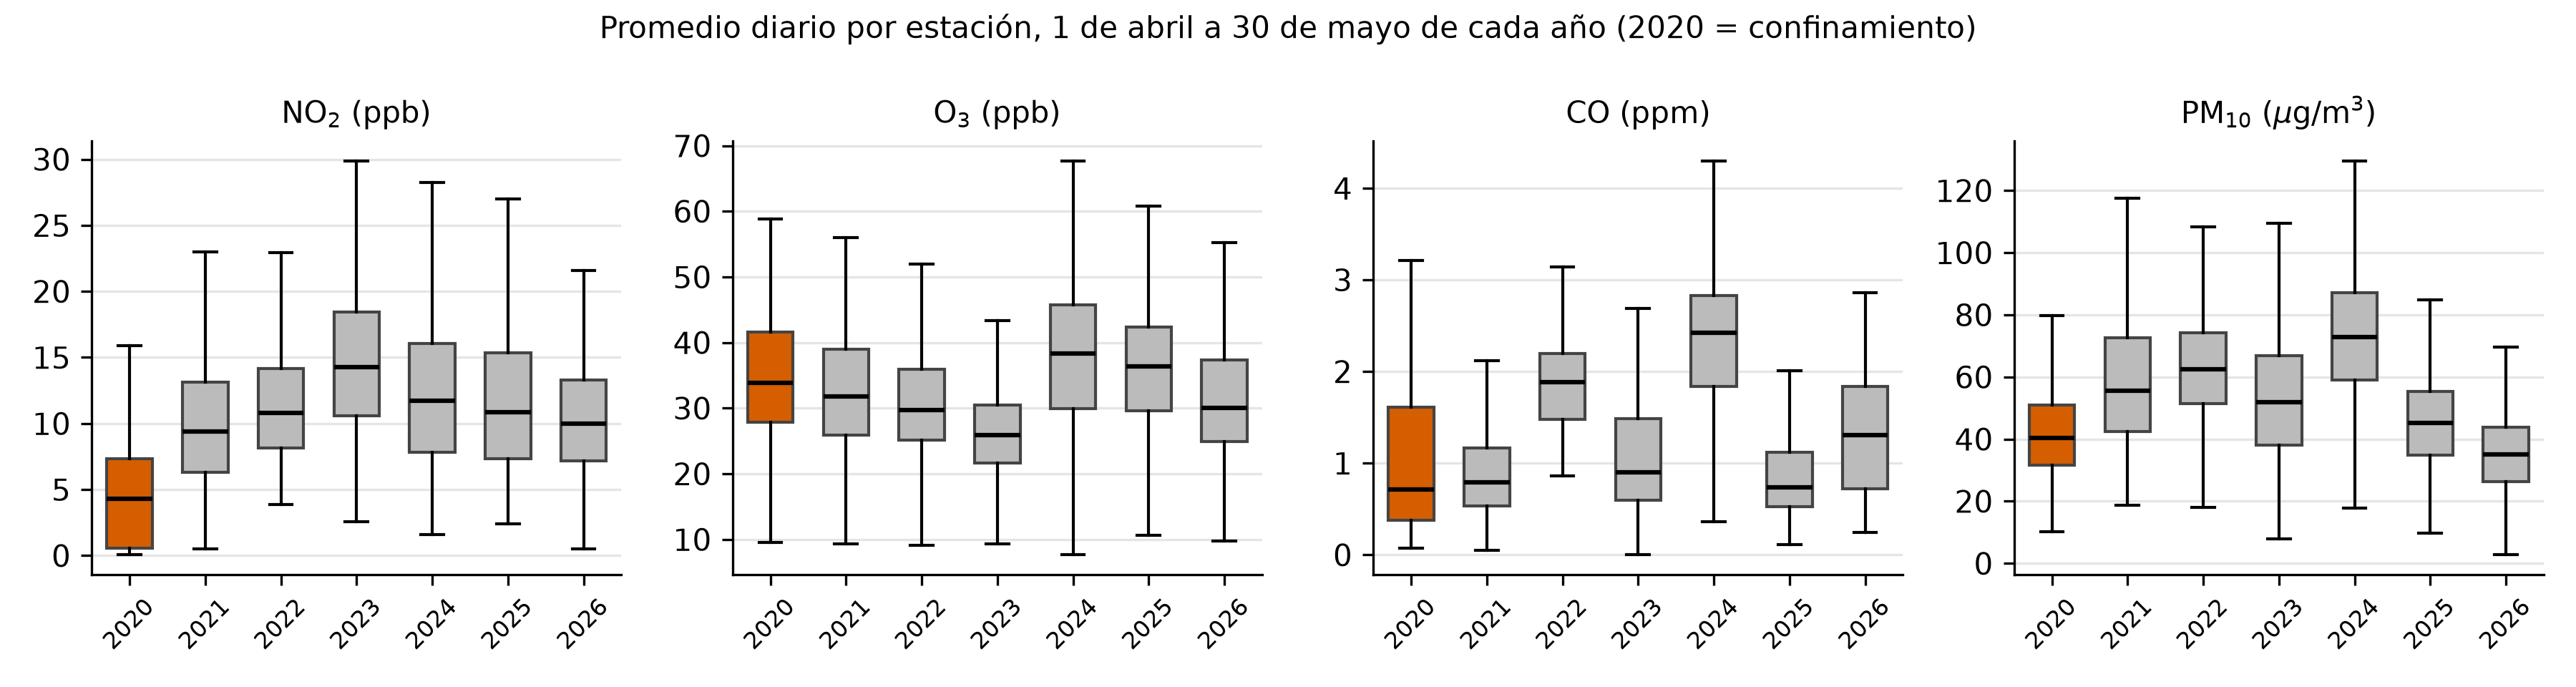
\includegraphics[width=0.82\textwidth]{figuras/fig_covid.png}
    \caption{Promedios diarios por estación del 1 de abril al 30 de mayo de cada año, para las 13 estaciones que operaban en 2020. En naranja, el confinamiento de 2020.}
    \label{fig:covid}
\end{figure}
 
Con el periodo de confinamiento de \citet{schiavo2023} (1 de abril a 30 de mayo 2020) y al revisar las bases de datos, se encontró que únicamente 13 estaciones operaban en 2020. Por lo tanto, para que la comparación entre años se usaron las mismas estaciones (ya que el resto de los años sí consideran 15 estaciones), se utilizaron solo esas 13. Con ellas, el NO$_2$ muestra un efecto claro, ya que su mediana fue alrededor de 4~ppb, contra 9.5--14~ppb en los demás años y toda la caja de 2020 queda por debajo de las del resto (Figura~\ref{fig:covid}). En el O$_3$ y el PM$_{10}$, 2020 queda dentro de la variación entre años, que es amplia (la mediana del PM$_{10}$ va de 35 a 73~$\mu$g/m$^3$ en las mismas fechas), por lo que su efecto no puede separarse sin controlar la meteorología, esta es una de las limitaciones que también son señaladas por \citet{schiavo2023}. En cuanto al CO, este alterna entre años de nivel alto y bajo, lo cual sugiere que el equipo que lo midió sufrió un cambio o un ajuste de calibración. Es por esto que se propone conservar 2020 con una variable indicadora del confinamiento, esto para estimar su efecto sobre la probabilidad de excedencia controlando por meteorología, la cual es la aportación frente a \citet{schiavo2023}. 
 
\section{Síntesis final}
\begin{itemize}[leftmargin=*]
    \item\textbf{Hallazgos.} Las excedencias dependen del contaminante, la estación, la hora, la temporada y la meteorología. El PM$_{10}$ rebasa la norma uno de cada cuatro días, sobre todo en invierno; el O$_3$ en tardes de sol y calor (como en primavera); y el NO$_2$, SO$_2$ y CO suelen rebasar la norma con menor frecuencia. Con menos actividad (fin de semana y el periodo de confinamiento) bajan los contaminantes de tráfico y sube el O$_3$. 
    \item \textbf{Relación con el objetivo.} La frecuencia de excedencias define el umbral de cada contaminante. La hora, el mes, el día, la estación y la meteorología son las covariables candidatas de la GPD y de la probabilidad de superar el umbral. Lo que justifica el enfoque de valores extremos es la diferencia entre la cola y el promedio observada. 
    \item \textbf{Limitaciones.} hasta 89~\% de faltantes de PM$_{2.5}$ en NE3 (78~\% en NO3) y 15--29~\% de NO$_x$ en varias estaciones, se encontraron dos estaciones sin datos en 2020. A su vez, se detectaron fallas de sensor solo en máximos, cambios de nivel del CO, los datos del 2025 incompletos y un análisis sin control de la meteorología. 
    \item \textbf{Análisis pendiente.} Desagrupar los excesos de un mismo episodio, definir los umbrales, resumir la meteorología a través de componentes principales, agrupar estaciones, y estimar el efecto del confinamiento por COVID. Una vez que se toma en cuenta este análisis a desarrollar, se busca ajustar la probabilidad de superar el umbral ya sea a través de una regresión logística o discriminante y la GPD con covariables como modelo base. Por consiguiente, se debe evaluar si el aprendizaje profundo la mejora con métricas de calibración y falsas alarmas. 
    \item \textbf{Camino para responder el objetivo} Para próximas entregas se experimentará con el uso de redes neuronales combolusionales para el cálculo de probabilidades de que los contaminantes superen un cierto umbral, capturando relaciones entre los datos. 
    \item \textbf{Nuevas preguntas.} ¿El O$_3$ se acumula viento abajo? ¿Los faltantes son más frecuentes durante los episodios altos? ¿Qué parte del PM$_{10}$ invernal se debe a inversiones térmicas y cuál a la falta de lluvia?
\end{itemize}
 

 


\pagebreak
 
\appendix

\section{Revisión de calidad de los datos}
\label{anexo:limpieza}
 
\begin{table}[H]
\centering
\small
\caption{Correcciones aplicadas a la base observada.}
\begin{tabular}{p{4.2cm}rp{2.6cm}p{5.6cm}}
\toprule
\textbf{Problema} & \textbf{Casos} & \textbf{Decisión} & \textbf{Razón} \\
\midrule
Valores negativos (excepto temperatura) & 232 & Faltante & Físicamente imposibles \\
RH entre 100 y 105~\% & 271 & 100~\% & Saturación del sensor \\
RH mayor a 105~\% & 12 & Faltante & Imposible (máximo de 714~\%) \\
PM$_{2.5}$ mayor que PM$_{10}$ & 33 & Ambos faltantes & Imposible; no se sabe cuál falló \\
Temperatura fuera de $[-10, 50]$~$^\circ$C & 430 & Faltante & Código $-9999$, errores y falla de 426~h en NTE \\
PM$_{10} \geq 999$~$\mu$g/m$^3$ & 5 & Faltante & Límite del instrumento (0--1000) \\
CO = 37~ppm (SE, 22/05/2024) & 1 & Faltante & Pico aislado de una hora \\
NO = 814--945~ppb (NO, 15/03/2022) & 3 & Faltante & Probable calibración: sin NO$_2$ ni CO \\
O$_3$ en SE2 (09/06/2021) & 8 & Faltante & Supera al resto de las estaciones \\
NO$_x \neq$ NO + NO$_2$ & 1{,}035 & Se conserva & 59~\% en CE: posible calibración \\
Registros duplicados & 0 & --- & --- \\
\bottomrule
\end{tabular}
\end{table}
 
Los valores extremos se conservaron cuando eran consistentes con otras variables, como el PM$_{2.5}$ de 763~$\mu$g/m$^3$ en la noche de Año Nuevo de 2023 o el pico de SO$_2$ de 404.7~ppb en SE3, cuyo decaimiento gradual corresponde a una nube de contaminación.
 
\section{Estadísticos descriptivos}
\label{anexo:estadisticos}
\begin{table}[H]
\centering
\small
\caption{Estadísticos de los contaminantes (datos horarios, 2020--2026).}
\begin{tabular}{lrrrrrr}
\toprule
\textbf{Contaminante} & \textbf{\% faltante} & \textbf{Media} & \textbf{Mediana} & \textbf{P$_{90}$} & \textbf{P$_{99}$} & \textbf{Asimetría} \\
\midrule
CO (ppm) & 13.4 & 1.36 & 1.2 & 2.46 & 3.95 & 1.53 \\
NO (ppb) & 16.9 & 11.89 & 5.0 & 27.4 & 105.0 & 6.56 \\
NO$_2$ (ppb) & 17.5 & 14.35 & 11.2 & 29.1 & 52.8 & 2.00 \\
O$_3$ (ppb) & 14.2 & 27.34 & 24.0 & 52.0 & 88.1 & 1.28 \\
PM$_{10}$ ($\mu$g/m$^3$) & 4.3 & 57.33 & 48.0 & 100.0 & 201.0 & 3.55 \\
PM$_{2.5}$ ($\mu$g/m$^3$) & 23.4 & 20.25 & 17.0 & 38.0 & 70.0 & 4.02 \\
SO$_2$ (ppb) & 14.6 & 4.94 & 3.9 & 8.2 & 20.2 & 12.09 \\
\bottomrule
\end{tabular}
\end{table}
 
 
\section{Datos faltantes por estación}
\label{anexo:faltantes}
\begin{figure}[H]
    \centering
    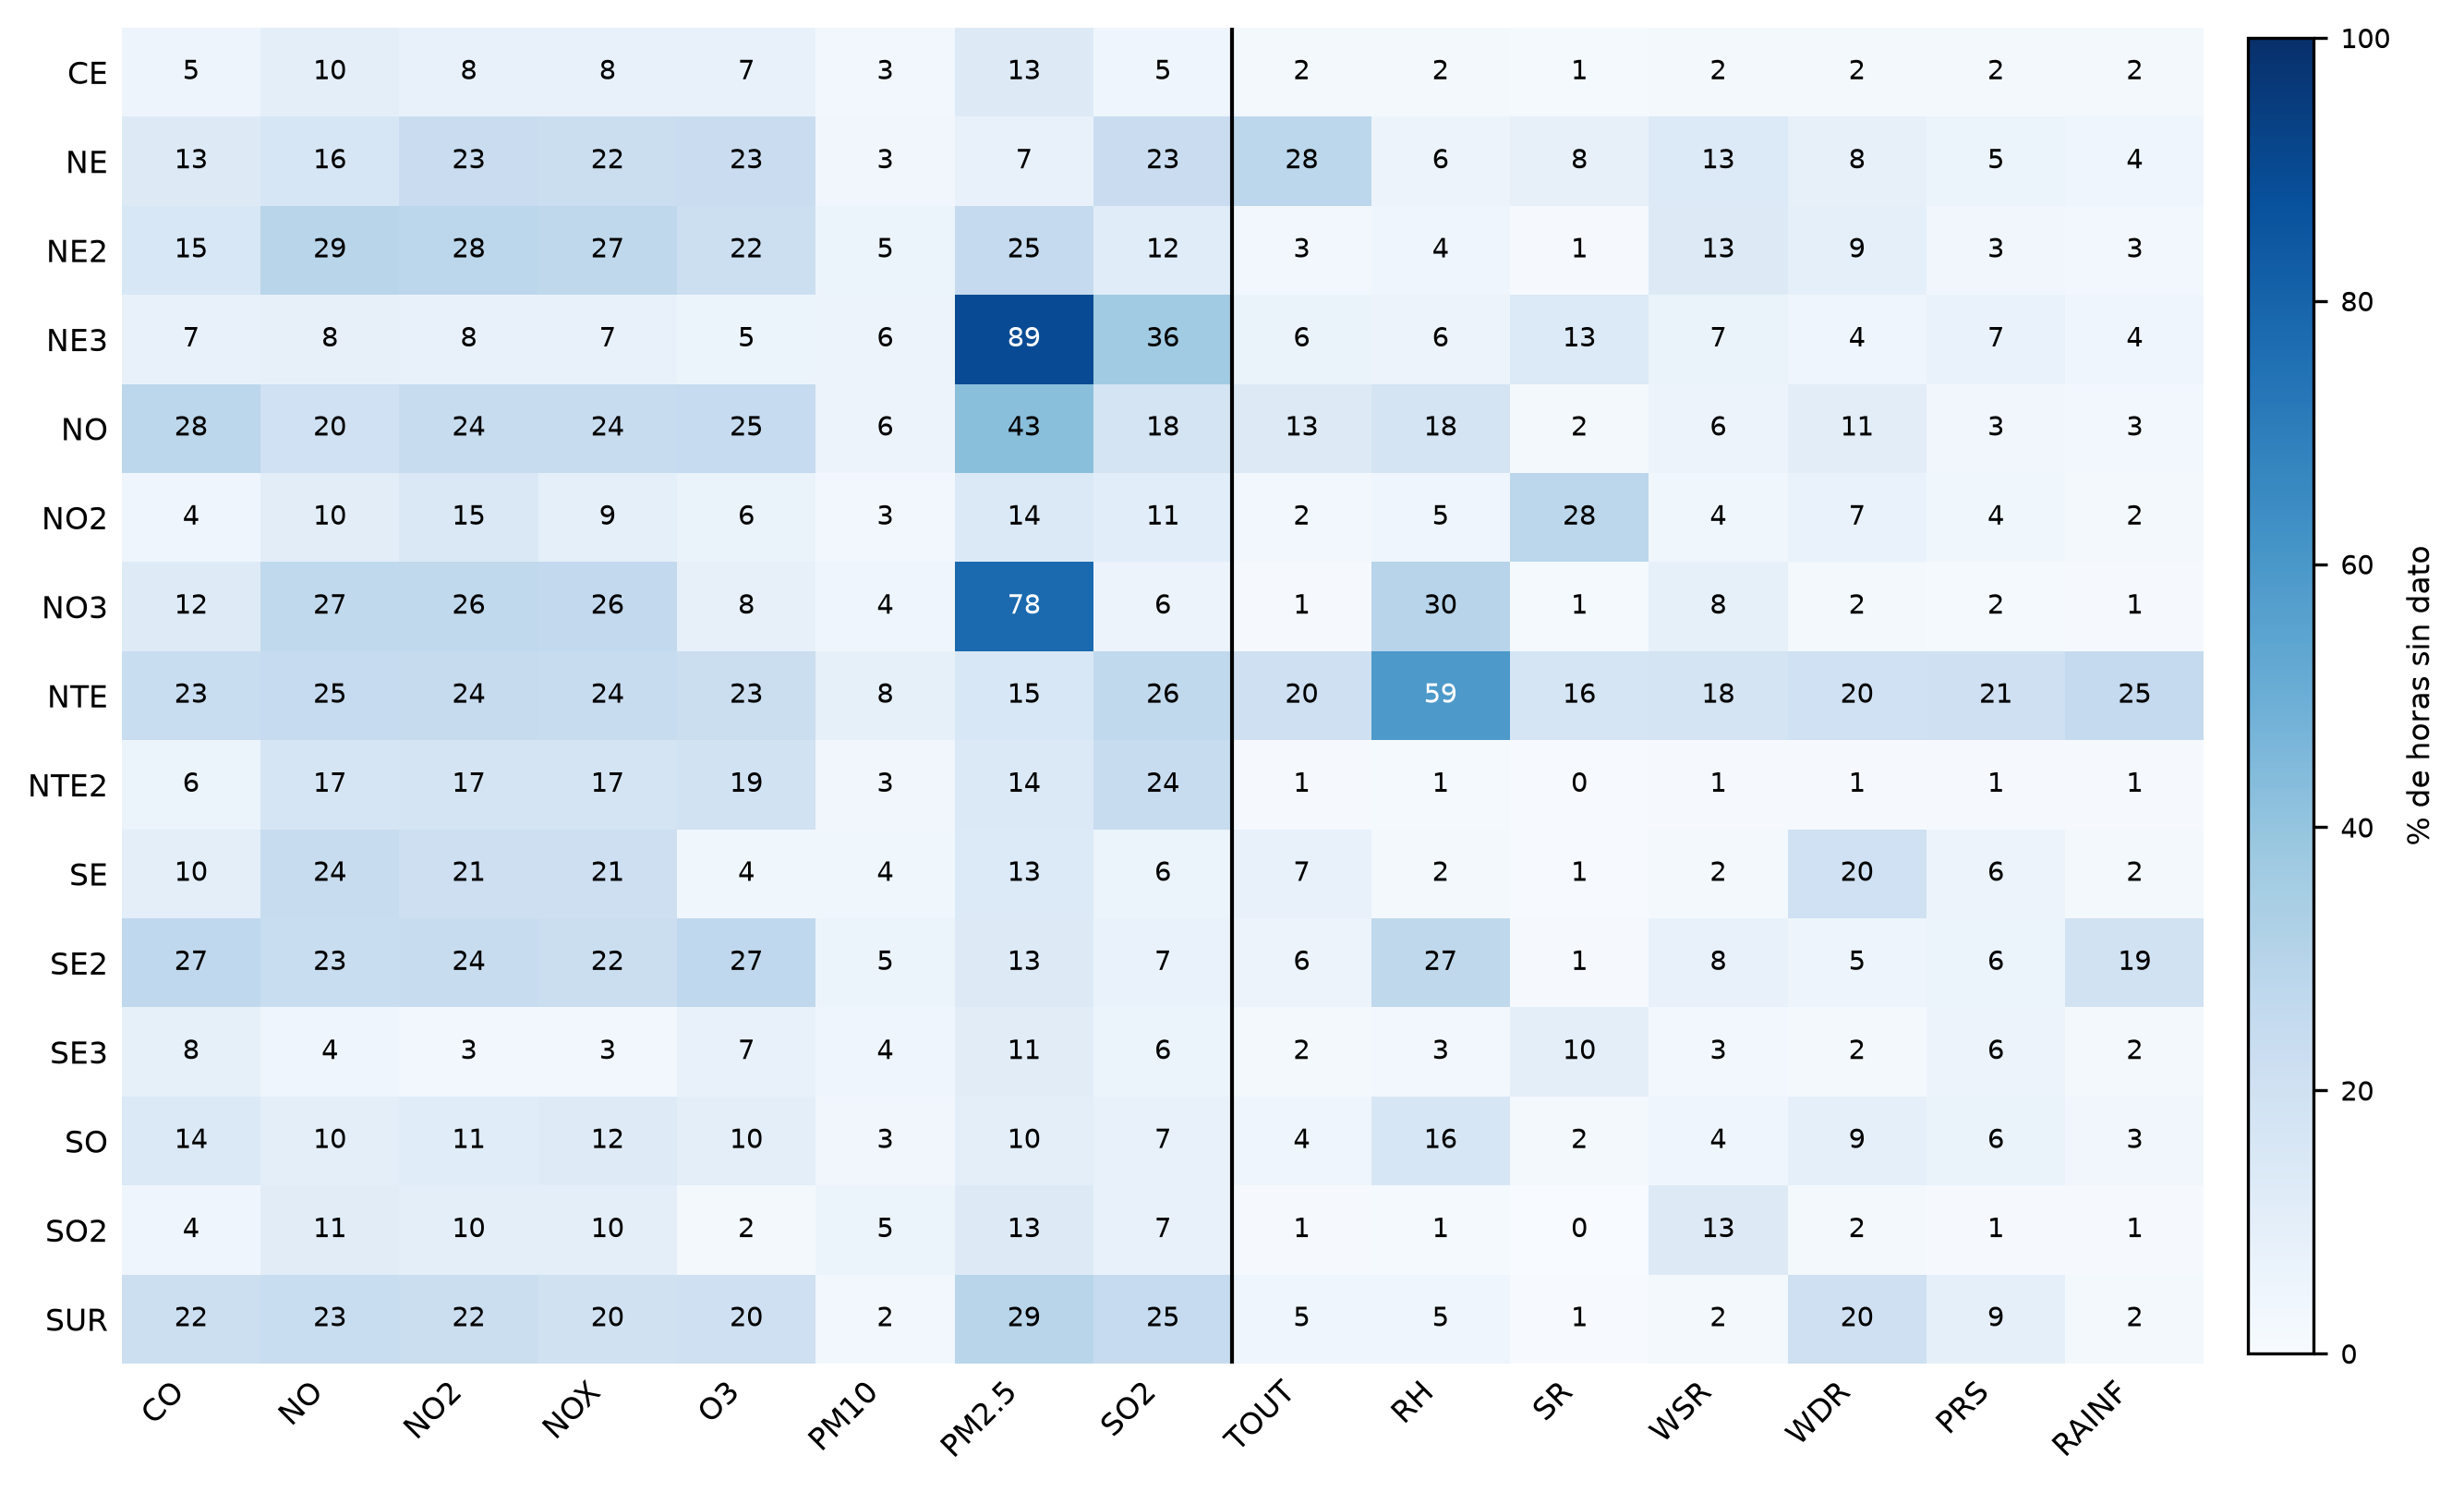
\includegraphics[width=0.9\textwidth]{figuras/fig_faltantes.png}
    \caption{Porcentaje de horas sin dato por estación y variable.}
\end{figure}
Los faltantes de NO, NO$_2$ y NO$_x$ coinciden en cada estación porque se miden con el mismo analizador. El PM$_{10}$ es la variable más completa (2--8~\%), y la estación NTE tiene faltantes de 15 a 25~\% en casi todas las variables, lo que indica periodos sin operación.
 
\section{Concentraciones por tipo de día}
\label{anexo:dias}
\begin{table}[H]
\centering
\small
\caption{Medianas horarias entre semana y en fin de semana.}
\begin{tabular}{lrrr}
\toprule
\textbf{Contaminante} & \textbf{Entre semana} & \textbf{Fin de semana} & \textbf{Cambio (\%)} \\
\midrule
CO (ppm) & 1.2 & 1.2 & $-1.7$ \\
NO (ppb) & 5.2 & 4.5 & $-13.5$ \\
NO$_2$ (ppb) & 11.8 & 9.9 & $-16.1$ \\
O$_3$ (ppb) & 23.0 & 25.0 & $+8.7$ \\
PM$_{10}$ ($\mu$g/m$^3$) & 50.0 & 45.0 & $-10.0$ \\
PM$_{2.5}$ ($\mu$g/m$^3$) & 17.0 & 16.3 & $-4.0$ \\
SO$_2$ (ppb) & 3.9 & 3.9 & 0.0 \\
\bottomrule
\end{tabular}
\end{table}
 
\section{Meteorología en los días de concentración más alta}
\label{anexo:p95}
Como el NO$_2$, el SO$_2$ y el CO casi nunca rebasan la norma, para comparar todos los contaminantes se tomó como umbral el percentil 95 (P$_{95}$) de sus promedios diarios por estación. La tabla muestra la mediana de cada variable meteorológica en los días sobre el P$_{95}$ menos la mediana en el resto de los días.
\begin{table}[H]
\centering
\small
\caption{Diferencia de medianas entre los días sobre el P$_{95}$ y el resto (promedios diarios por estación).}
\vspace{5pt}
\begin{tabular}{lrrrrrr}
\toprule
\textbf{Contaminante} & \textbf{P$_{95}$} & \textbf{Temp.} & \textbf{Humedad} & \textbf{Radiación} & \textbf{Viento} & \textbf{Días con} \\
 & & \textbf{($^\circ$C)} & \textbf{(\%)} & \textbf{(kW/m$^2$)} & \textbf{(km/h)} & \textbf{lluvia (pp)} \\
\midrule
CO (ppm) & 2.8 & $-4.0$ & $-2.4$ & $-0.01$ & $-0.9$ & $-5.4$ \\
NO$_2$ (ppb) & 31.2 & $-5.2$ & $-9.0$ & $-0.03$ & $-2.8$ & $-5.3$ \\
O$_3$ (ppb) & 43.8 & $+2.5$ & $-13.0$ & $+0.06$ & $+0.4$ & $-5.5$ \\
PM$_{10}$ ($\mu$g/m$^3$) & 109.6 & $-3.8$ & $-13.4$ & $-0.02$ & $-1.9$ & $-8.0$ \\
PM$_{2.5}$ ($\mu$g/m$^3$) & 39.8 & $-3.2$ & $+0.7$ & $-0.02$ & $-2.9$ & $-5.3$ \\
SO$_2$ (ppb) & 9.8 & $-2.8$ & $-3.4$ & $+0.01$ & $-1.4$ & $-3.1$ \\
\bottomrule
\end{tabular}
\end{table}
Los contaminantes primarios (CO, NO$_2$, PM$_{10}$, PM$_{2.5}$ y SO$_2$) tienen sus días más altos con menos temperatura, menos viento y menos lluvia, lo que apunta a la acumulación en días fríos. El O$_3$ es la excepción, ya que sus días altos son más cálidos y con más radiación, como corresponde a un contaminante secundario de origen fotoquímico. Se debe considerar que en todos, los días altos tienen menos lluvia. A diferencia del PM$_{10}$, en el PM$_{2.5}$ la humedad casi no cambia, por lo que la meteorología de cada contaminante debe modelarse por separado.
 
 
\section{Correlación entre variables}
\label{anexo:correlacion}
\begin{figure}[H]
    \centering
    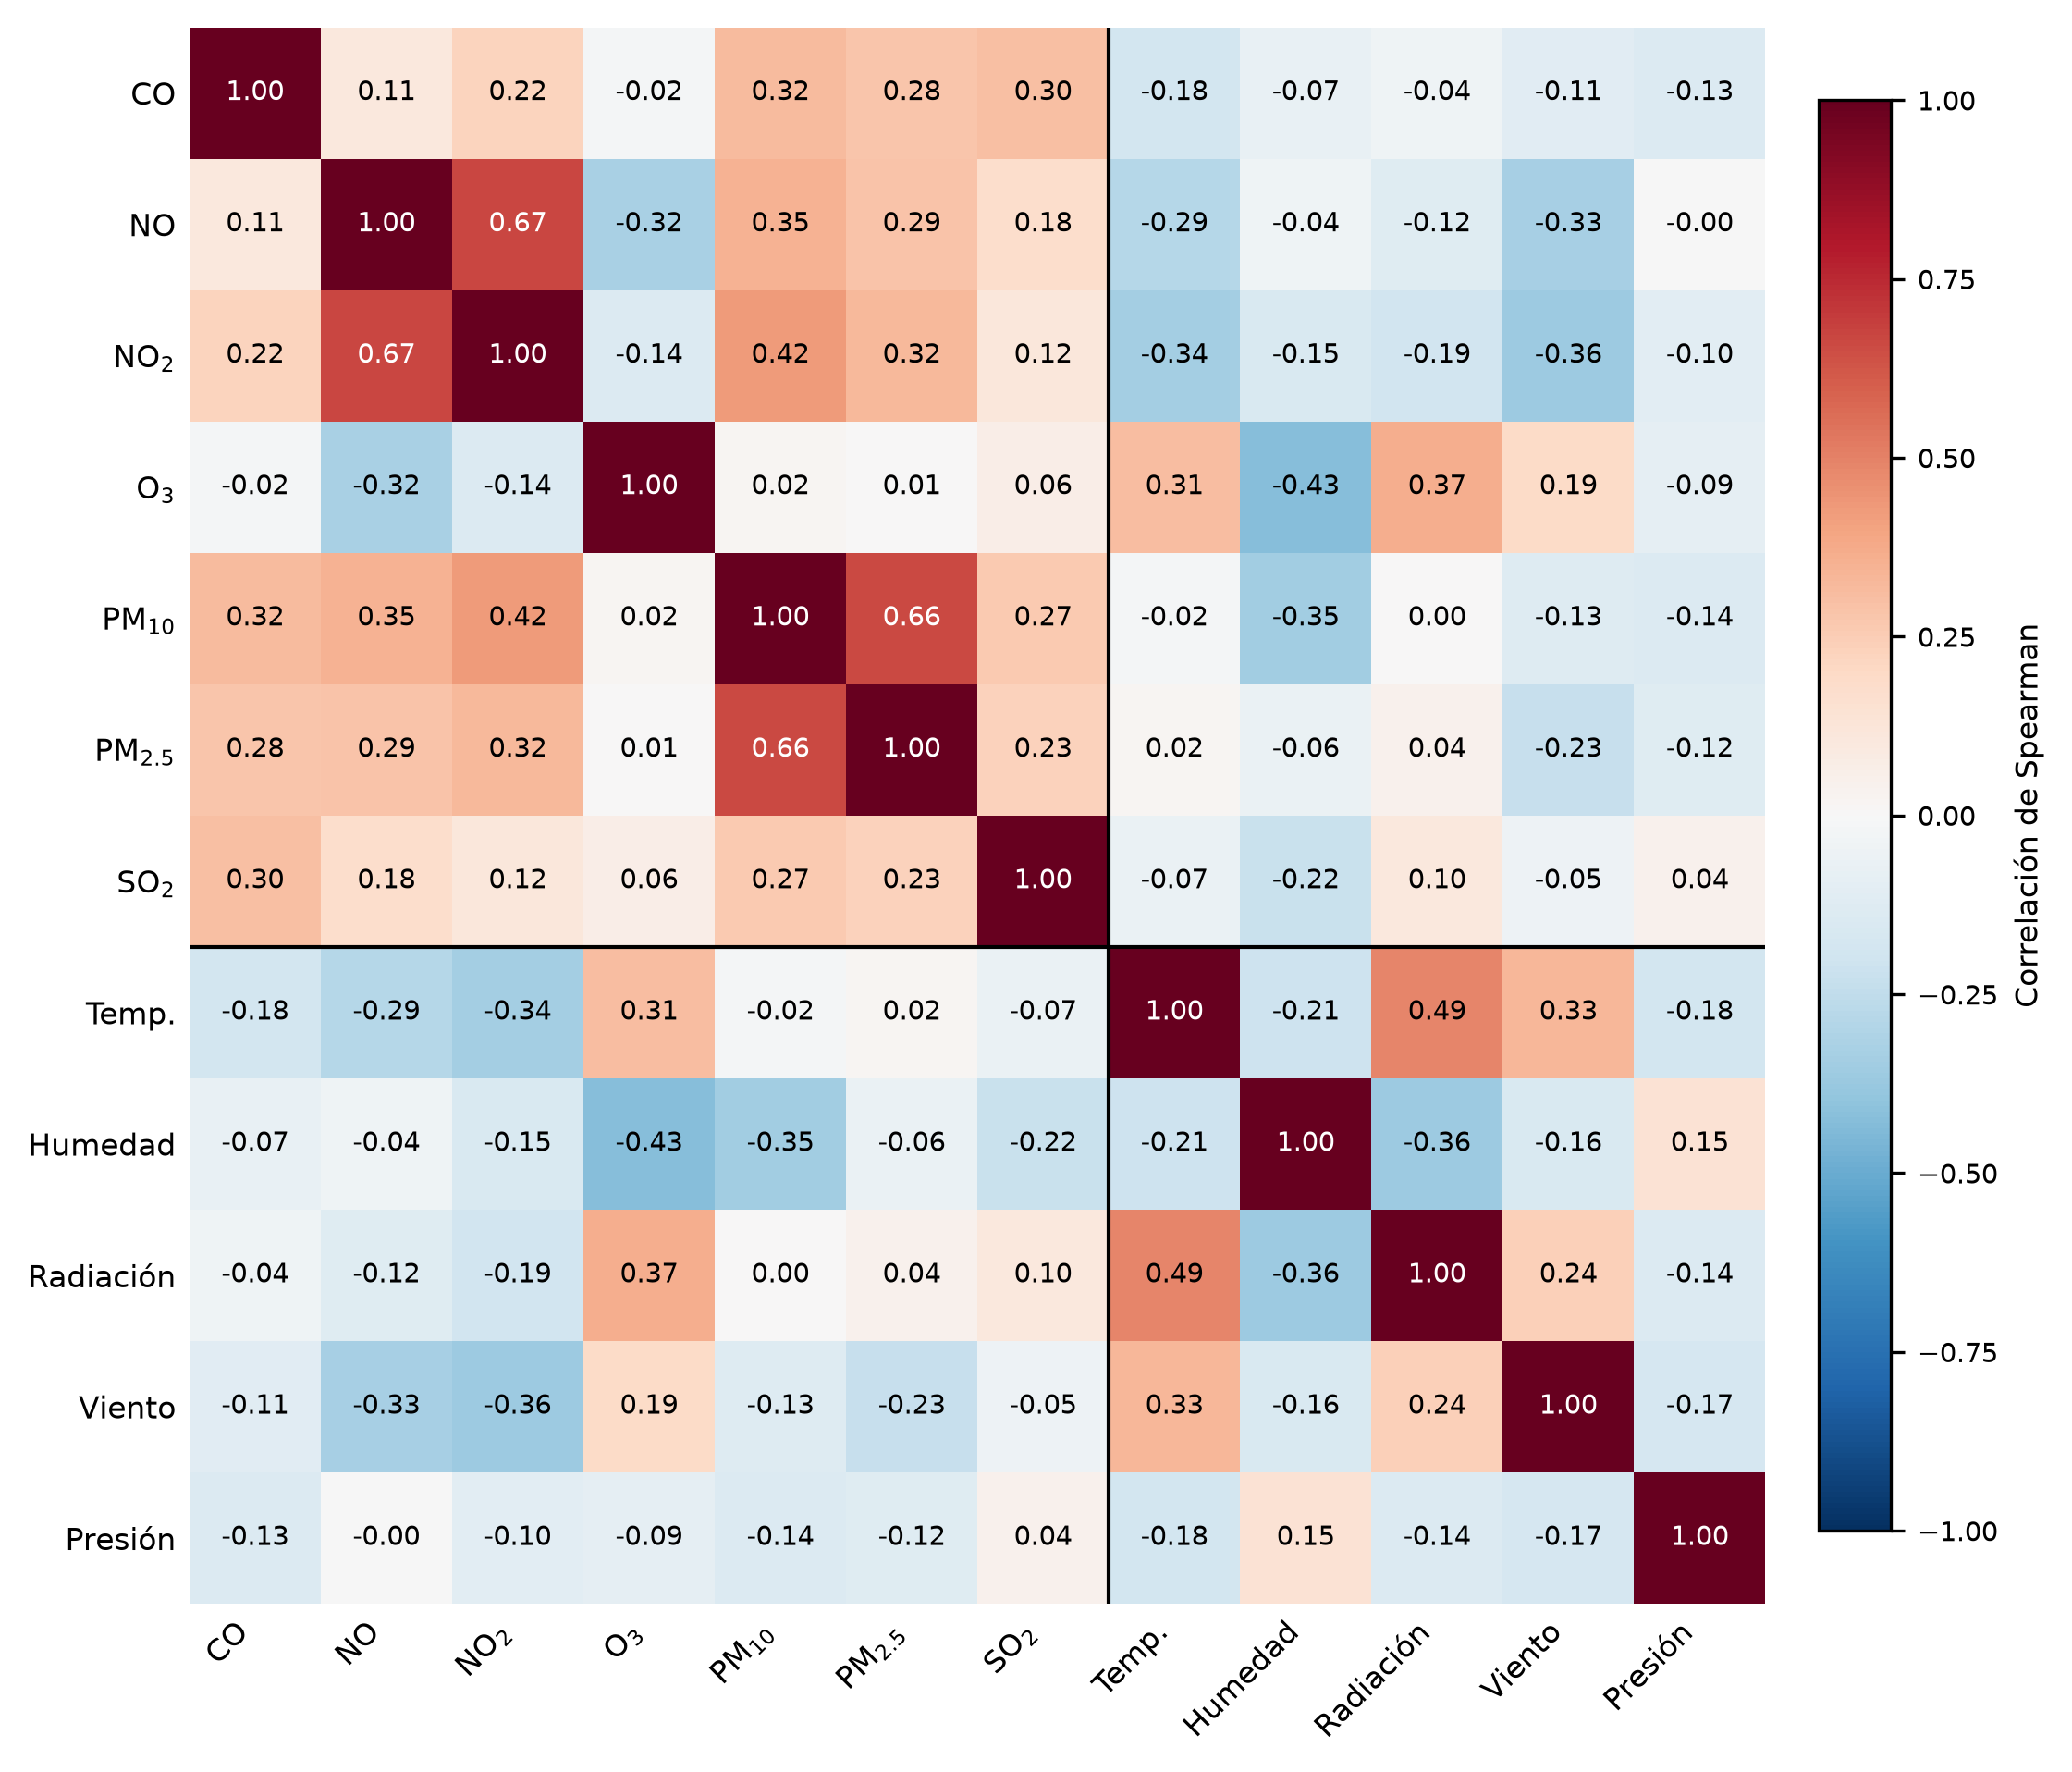
\includegraphics[width=0.75\textwidth]{figuras/fig_correlacion.png}
    \caption{Correlación de Spearman entre promedios diarios por estación.}
\end{figure}

\section{Tabla de excedencias por días distintos} 
\label{anexo:excedencias}
\begin{table}[H]
\centering
\small
\begin{tabularx}{\textwidth}{>{\raggedright\arraybackslash}p{2.8cm} >{\centering\arraybackslash}X >{\centering\arraybackslash}X >{\centering\arraybackslash}X >{\centering\arraybackslash}p{3cm}}
\toprule
Norma & \textbf{Periodos totales} & \textbf{Periodos con excedencias en todas las estaciones} & \textbf{Días distintos con excedencias} & \textbf{\% periodos con excedencias} \\
\midrule
CO 8h móvil & 661,303 & 35 & 35 & 0.01 \\
NO$_2$ 1h & 631,026 & 220 & 80 & 0.03 \\
O$_3$ 1h & 656,342 & 5763 & 595 & 0.88 \\
PM$_{10}$ 24h & 30,367 & 7717 & 2150 & 25.41 \\
PM$_{2.5}$ 24h & 24,075 & 1039 & 1789 & 4.32 \\
SO$_{2}$ 1h & 653,043 & 301 & 168 & 0.05 \\
SO$_{2}$ 24h & 26,902 & 4 & 569 & 0.01 \\
\bottomrule
\end{tabularx}
\end{table}

\section{GitHub}

El código usado para la preparación de los datos en este trabajo puede ser accedido mediante el siguiente vínculo:

\url{https://github.com/RicardoSalgadoB/MultiReto}

\section{Declaratoria del uso de IA}

Los usos de la Inteligencia Artificial Generativa en este trabajo incluyen:

\begin{itemize}
    \item Se usó Claude Sonnet 5.5 (Esfuerzo alto) para generar ideas y revisar la literatura respecto a la generación de grafos en el contexto geoespacial. Para todos los enfoques propuestos se revisó la literatura citada y la implementación particular para cada caso.
    \item Se usó la IA integrada en el editor de \LaTeX \textit{Prism} para agregar de manera rápida las tablas generadas en la ejecución del código en este documento. En todo caso se confirmó que el contenido se hubiese copiado de manera correcta.
\end{itemize}

Para todos los usos anteriores, se confirma que los miembros del equipo revisaron y verificaron las salidas y que se asume la responsabilidad del contenido final entregado.

\pagebreak

\nocite{*}
\bibliographystyle{apacite}
\bibliography{references}
\end{document}